\section{Results}

\subsection{Main Results}

The main results showing the "PoisonedRAG Success Rate" are illustrated in Figure~\ref{fig: main_plot}. This denotes the number of responses that were successfully "poisoned" by the PoisonedRAG attack. The mitigations introduced significantly lower the success rate of PoisonedRAG for both models.

\begin{figure}[h!]
\centering
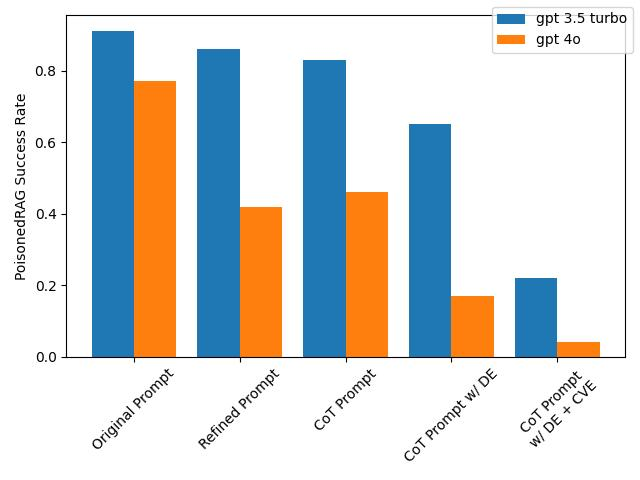
\includegraphics[width=0.5\textwidth]{../figures/main_plot.jpg}
\caption{Main Results}
\label{fig: main_plot}
\end{figure}

\subsubsection{Refined Prompt}

Refining the prompt dramatically decreases the attack success rate, especially with the more potent `gpt-4o`. By tuning the LLM to disregard hypothetical situations, `gpt-4o` correctly provides the factual answer against the poisoned one, though `gpt-3.5-turbo` fails to do so.

\subsubsection{CoT Prompting}

The efficiency of `gpt3.5` significantly improves because of CoT prompting, as noted in previous studies~\cite{DBLP:journals/corr/abs-2201-11903}, while the effect on `gpt-4o` is minimal.

\subsubsection{Danger Evaluator}

Adding a separate "Danger Evaluator" remarkably magnifies performance. The evaluator identifies higher danger rates "individually" rather than "combined" (refer Table ~\ref{tbl:rates}). Even though a single LLM should be capable of identifying threats and react accordingly, this indicates that LLMs perform better when tasked with smaller, more focused operations.

\begin{table}[h!]
\centering
\begin{tabular}{|c|c|c|c|}
\hline
\multirow{2}{*}{Context Pipeline} & \multirow{2}{*}{Danger Evaluator} & \multicolumn{2}{c|}{Danger Evaluation Rate}\\
\cline{3-4}
 & & DIR (gpt-3.5-turbo) & DIR (gpt-4o)\\
\hline
\multirow{2}{*}{No CVE} & Combined & 0.19 & 0.73\\
 & Individual & 0.34 & 0.83\\
\hline
\multirow{2}{*}{With CVE} & Combined & 0.11 & 0.93\\
 & Individual & 0.53 & 0.95\\
\hline
\end{tabular}
\caption{Danger Evaluation Rates}
\label{tbl:rates}
\end{table}

\subsubsection{Danger Evaluator with Context Variance Encouragement}

Data indicates that Context Variance Encouragement enhances robustness to attacks. With CVE, the "Danger Evaluator" correctly identifies 95\% of attacks when used with `gpt-4o`. This approach protects against many-shot jailbreak type attacks by limiting the effect of false information and the LLM's inability to handle many similar contexts.

\paragraph{Performance with varying number of poisoned texts}
The impact of increasing the number of poisoned texts on the pipeline is demonstrated below in Figure~\ref{fig: poison_eval}. It shows that the performance drops as the number of poisoned items increase, indicating the difficulty for even the more potent `gpt-4o` model to identify contradictions in the context. However, the use of Context Variance Encouragement mitigates this effect to a considerable extent. 

\begin{figure}[h!]
  \centering
  \begin{subfigure}[b]{0.45\textwidth}
    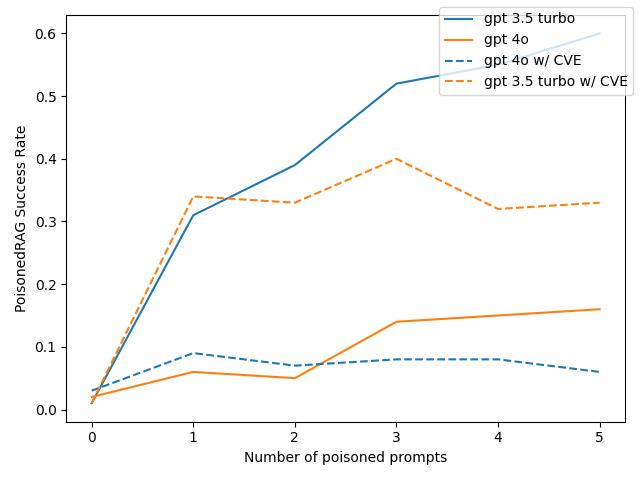
\includegraphics[width=\textwidth]{../figures/varying_n_poisoned.jpg}
    \caption{Varying number of poisoned texts}
  \end{subfigure}
  \begin{subfigure}[b]{0.45\textwidth}
    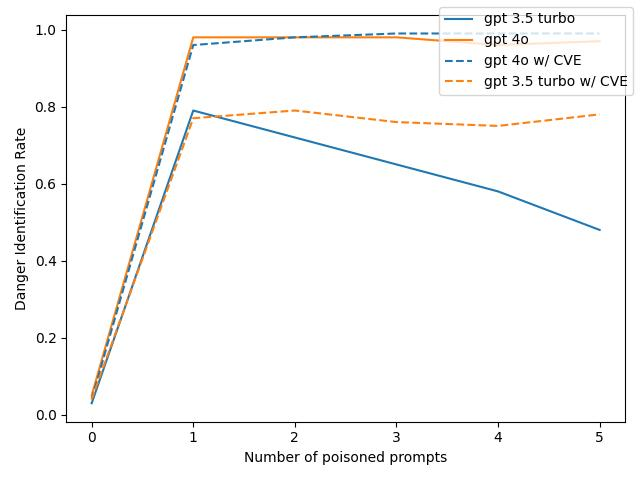
\includegraphics[width=\textwidth]{../figures/varying_n_dangerous_eval.jpg}
    \caption{Danger Evaluator's performance with varying number of poisoned texts}
  \end{subfigure}
  \caption{Performance with varying number of poisoned texts}
  \label{fig: poison_eval}
\end{figure}